
\emph{Global} formulae relate several hidden ground atoms. We use them for two 
purposes: to ensure consistency between the decisions of all SRL stages and to 
capture some of our intuition about the task. We will refer to formulae that 
serve the first purpose as \emph{structural constraints}. 

For example, a structural constraint is given by the (deterministic) formula
\[role(p,a,r) \Rightarrow hasRole(p,a)\]
which ensures that, whenever the argument $a$ is given a label $r$ with respect 
to the predicate $p$, this argument must be an argument of $a$ as denoted by 
\emph{hasRole(p,a)}. Note that this formula by itself models the traditional 
``bottom-up'' argument identification and classification pipeline: it is 
possible to not assign a role $r$ to an predicate-argument pair $(p,a)$ proposed 
by the identification stage; however, it is impossible to assign a role $r$ to 
token pairs $(p,a)$ that have not been proposed as potential arguments.

One example of another class of structural constraints is 
\[
hasRole(p,a)\Rightarrow\exists r.role(p,a,r)
\]
which, by itself, models an inverted or ``top-down'' pipeline. In this Figure 
\ref{fig:global2} illustrates the structural formulae we use in form of a Markov 
Network.

The formulae we use to ensure consistency between the remaining hidden 
predicates are omitted for brevity as they are very similar to the bottom-up and 
top-down formulae we presented above.

For the SRL predicates that perform a labelling task (\emph{role} and 
\emph{sense}) we also need a structural constraint which ensures that not more 
than one label is assigned. For instance,
\[
(role(p,a,r_1) \wedge r_1 \neq r_2 \Rightarrow \neg role(p,a,r_2)  )
\]
forbids two different semantic roles for a pair of words. 

The global formulae that capture our intuition about the task itself can be 
further divided into two classes. The first one uses deterministic or 
\emph{hard} constraints such as
\begin{eqnarray*}
 &role\left(p,a_{1},r\right)\wedge \neg mod\left(r\right)\wedge a_{1}\neq a_{2}  \Rightarrow\\
  & \neg role\left(p,a_{2},r\right)
\end{eqnarray*}
which forbids cases where distinct arguments of a predicate have the same role 
unless the role describes a modifier.

The second class of global formulae is \emph{soft} or nondeterministic. For 
instance, the formula
\begin{eqnarray*}
  & lemma(p,+l) \wedge ppos(a,+p)  \\
  & \wedge hasRole(p,a)  \Rightarrow sense(p,+f) 
\end{eqnarray*}
is a soft global formula. It captures the observation that the sense of a verb 
or noun depends on the type of its arguments. Here the type of an argument token 
is represented by its POS tag.

\begin{figure}
\begin{center}
   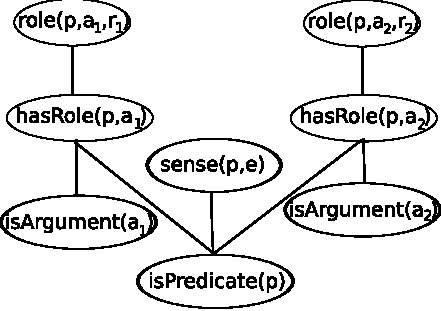
\includegraphics[scale=.70]{GlobalFormula2}
\end{center}
\caption{Markov Network that illustrates the structural constraints we use.}
\label{fig:global2}
\end{figure}




